\section{Motivation}
\label{sec:motivation}

\subsection{Command Semantics}
\label{subsec:semantics}

% VALUE: the CP semantics, measured on the existing prefill's own operators, say where concurrency can come from: not from queued commands, but from one command that issues both groups' work before it waits on either
To find where concurrency can come from, we measure how the CP turns instruction streams into overlap on the existing prefill's own operators, pairing one attention operator on columns 0 and 7 with one GEMM operator on columns 1--6.
Every composed command here produces outputs bit-identical to those of the operators run alone.

\begin{figure}[t]
    \centering
    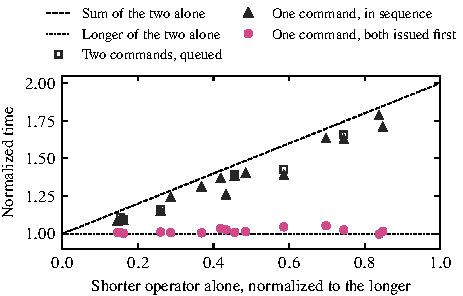
\includegraphics[width=\linewidth]{fig/pairs.pdf}
    % VALUE: queued commands take the sum of the two operators, one command that issues both before waiting takes the longer one
    \caption{Median time of one attention and one GEMM operator on disjoint column groups, normalized to the longer operator alone, over 20 runs per pair. Holding both streams in one command saves one dispatch floor against the sum.}
    \label{fig:pairs}
\end{figure}

\textbf{Queued Commands.}
% VALUE: the runtime gives no overlap across commands, and placing two operators in one command is itself neutral, so overlap must come from within a command
Two commands queued on one hardware context, with no wait between them, take as long as one command that holds both streams in sequence, within 3\% on each of the seven pairs where we queue them (Figure~\ref{fig:pairs}).
Holding both streams in sequence in one command takes the sum of the two operators' times minus one dispatch floor, within 2\%, so placing two operators in one command is itself neutral.
This is why packing several operators into one dispatch, which is standard practice for amortizing launch cost, as in CUDA Graphs~\citep{nvidia-cudagraphs}, XRT's run lists~\citep{xrt-repo}, and MLIR-AIR's multi-launch programs~\citep{wang2026mlirair}, removes dispatch cost on the NPU but creates no overlap.
% SOURCE: queued / in-sequence = 1.007-1.029 on 7 pairs (amd-npu 17f7ec3 prefill-overlap/ovl4/, lab-prefill-overlap (5)b); in-sequence / (A + G - F) = 0.996-1.021 over 17 pair runs (ovl/, ovl2/ at 8f13e05 and ovl4/; report.txt H1 column).
% SOURCE: XRT run list, /opt/xilinx/xrt/include/xrt/experimental/xrt_kernel.h:21 (XRT 2.25.0); MLIR-AIR stitch_elf (vault src-mlir-air-llms).

\textbf{Concurrent Issue.}
% VALUE: one command that issues both groups' work before it waits on either runs them concurrently at nearly the longer one's time; the small cost appears when both read DRAM near the cap
When one command issues all of the GEMM's work, then the attention operator's stream, and only then the GEMM's synchronizations, the two operators run concurrently.
Such a command takes 1.00--1.06 times the longer operator's time on 9 pairs that cover three GEMM shapes and attention over chunks 0 to 15 (Figure~\ref{fig:pairs}).
On six further pairs with other shapes and chunks, the overlap hides 90--96\% of the shorter operator's work, after excluding the dispatch floor that the merge already saves.
The overlap costs most when the pair's combined DRAM read rate approaches the read cap, at about 95\% of the cap measured in the same batch.
The serial execution of the existing prefill is therefore a property of how its commands are composed, not of the array or its configuration.
% SOURCE: interleaved / max(A, G) = 0.998-1.058 over 10 pair runs = 9 pairs (c8 + lm measured twice, 1.054 and 1.058; the figure keeps each pair's first measurement); GEMM shapes up, LM head chunk, down; attention chunks 0, 4, 8, 12, 15 (lab-prefill-overlap (3)).
% SOURCE: hidden fraction of the shorter operator's work, (in-sequence - interleaved) / (min(A, G) - F) = 0.90-0.96 on 2+qkv, 6+o, 11+gate, 14+qkv, 6+gate, 11+o (lab-prefill-overlap (5)a).
% SOURCE: DRAM rate during the interleaved command 52.2 GB/s against a same-batch 8x2 cap of 53.9-55.3 GB/s for c8 + lm, the costliest overlap (1.054-1.058) (lab-prefill-overlap (3)).

\textbf{Synchronization Order.}
% VALUE: because the CP is in order, a wait on one group delays the issue of every other group's work; the attention measurement of Section 4.1 isolates this effect, so the instruction order is a scheduling decision of its own
Since the CP executes in order, a synchronization on one group delays every later issue, including the issue of another group's work.
The existing attention operator isolates this effect (Section~\ref{subsec:losses}): its two columns carry equal work, yet alternating their segments lowers its device time to $0.67\times$ at 2{,}048 tokens with the same instructions.
The CP's instruction order, and not only the assignment of operators to commands, is therefore a scheduling decision.
% SOURCE: vault lab-prefill-overlap (4)-(5)c; Section 4.1 carries the numbers.

\textbf{Hardware Contexts.}
% VALUE: a second hardware context gives no concurrency here: the driver's source allocates every context the whole array and shares it in time, and narrower partitions would need contiguous columns, rebuilt designs, and a host round trip at every dependence, so concurrency comes from within one command
Two hardware contexts on disjoint partitions are the obvious alternative, but the driver's source shows that every hardware context on our platform is allocated all eight columns, so co-resident contexts share one partition in time, and measurement agrees: a one-column design submitted to two contexts at once takes 1.97$\times$ as long as on one alone, the same as queuing both on one context, although the pair draws half the DRAM read cap and so could have run side by side.
% SOURCE: amd-npu d8c63fb1 roofline/two-ctx-hold/two_ctx.json (registration lab-prefill-overlap (33), amd-npu 2171857e, tests 724b2f3b first; outputs committed before reading): rho 1.970, 95% bootstrap CI [1.955, 1.976], same-context ratio 1.970; medians solo 19.76 / 19.81 ms, pair 39.10 ms, same 39.09 ms; two 1x1 streams draw ~27 GB/s against an 8x2 cap of 54.7-54.9 GB/s in the same hold; verdict TEMPORAL CONFIRMED by the registered rule (vault lab-prefill-overlap (34)); verified from the bare by aie-cosched-c8.
Even where narrower partitions are allowed, a partition spans contiguous columns, whereas the existing attention sits on columns 0 and 7, so each group would need its own rebuilt design.
Every dependence between attention and a GEMM would then cross the host, which waits on one context before it submits to the other.
Concurrency on the array therefore comes from within one command, which needs no rebuild and no change to the driver or firmware.
% SOURCE: amdxdna 2.25.0 (loaded module 2.25.0_20260922, NPU Strix Halo 1022:17f0 rev 11, firmware 1.1.2.65): every firmware protocol the driver accepts on this device enables AIE2_TEMPORAL_ONLY (npu4_regs.c:94-106, the table npu5 shares), and aie2_alloc_resource (aie2_ctx.c:604-608) then requests start column 0 and all columns for every context, which the solver shares as one partition (vault lab-prefill-overlap (31)).
% SOURCE: contiguous partitions, separate 6- and 2-column builds with attention moved onto adjacent columns, and the host round trip (vault lab-prefill-overlap (1)).
% DECISION: the temporal sharing is stated from the driver's source with the driver named; a two-context behavioural check is registered and not run, so it is never worded as a measurement.


% MOVED from the former findings section: the measurements that motivate the work
\subsection{The Idle Array}
\label{subsec:losses}

\begin{figure}[t]
    \centering
    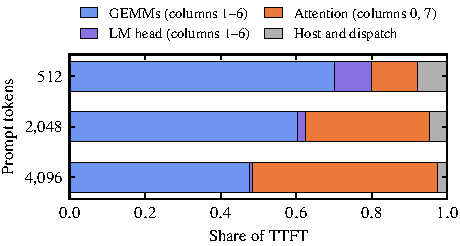
\includegraphics[width=\linewidth]{fig/busy.pdf}
    % VALUE: in the existing prefill, attention's share grows with prompt length, and each column group idles while the other computes
    \caption{Share of TTFT of the existing Llama-3.2-1B prefill by prompt length. Device-busy parts are each operator's time when dispatched alone, less the dispatch floor, summed over the prefill.}
    \label{fig:busy}
\end{figure}

\textbf{Column Groups in Prefill.}
% VALUE: the existing prefill issues one operator per command, so its column groups take turns; the device is busy almost all the time, but on one group at a time, and attention's growing share is time the GEMM columns sit idle
The existing prefill issues one operator per command, which amounts to about 1{,}500 commands for a 2{,}048-token prompt.
Figure~\ref{fig:busy} shows the resulting split of TTFT: device-busy time accounts for 92--97\% of it, and attention's share grows from 12\% to 49\% between 512 and 4{,}096 tokens.
Because the commands run in submission order, columns 1--6 idle while attention runs, and columns 0 and 7 idle while the GEMMs run, although neither group consumes the other's current work.
The device is thus busy almost all of the time, but on only one column group at a time.
% SOURCE: commands = 16 layers x chunks x 6 + 11 LM-head commands = 1,547 at 2,048 tokens (vault lab-prefill-census (1)).
% SOURCE: amd-npu e3acc8a prefill-e2/decomp.txt via figs/make_figs.py: busy = isolated time - dispatch floor = 92/95/97% of TTFT at 512/2k/4k; of TTFT, attention 12.2/32.9/49.1%, GEMMs 70.1/60.3/47.6%, LM head 9.7/2.1/0.8%.
% SOURCE: serial execution, the isolated busy times sum to at most TTFT (vault lab-prefill-device (4)); queued commands do not overlap (Section 3.1).

\textbf{Columns of One Operator.}
% VALUE: the same loss occurs inside one operator: the existing attention stream starts column 7 only after waiting on column 0, which costs a third of attention's device time
The existing attention stream issues column~7's inputs only after two synchronizations on column~0's key and value transfers, which complete when column~0 is about half done.
Alternating the two columns' segments, so that both columns start before the CP waits on either, reduces attention's device-busy time to $0.67\times$ that of the existing order at each of the seven chunks we measure between chunks 2 and 14 of a 2{,}048-token prompt, with bit-identical outputs.
Each column's half alone takes the same time within 1\%, so the difference comes from the CP's instruction order rather than from an imbalance of work.
Since attention's share grows with the prompt, this loss grows with it, and with the cached context: on a 4{,}096-token append to a 16{,}384-token context, the CP blocks at the existing attention stream's column synchronizations for 11.6--12.2\,s, 2.20--2.32$\times$ the 5.26\,s it blocks once the columns alternate, and those waits account for all of the 6.3--6.9\,s by which the existing program is slower, with device work and host gaps unchanged.
% SOURCE: amd-npu 596db771 (record-timer hold, registered lab-split-sweep (39); outputs d937fb68 committed before reading; reader fixed test-first d5ff7b70), Llama-3.2-1B S2 16,384 + 4,096, 5 reps, all in the shipped program's usual mode (12.55-13.16 s): ship - shipar 6,306-6,913 ms per rep, of which CP blocking at attention's column syncs 6,336-6,950 ms; attention device time outside blocking, host gaps and GEMM device time each within 3 ms; residual -33 to -37 ms; shipar blocking 5,264.0 ms every rep (vault lab-split-sweep (40)). The shipped program's rarer fast mode (8.86 s, lab-split-sweep (18)) did not appear in this hold or in (31)'s 80 reps.
% SOURCE: decoded from the shipped a_32_4_0_0 stream, mid-stream synchronizations at ops 70, 75 (column 0) and 92, 97 (column 7); column 7's issue (ops 81-91) follows column 0's two mid-stream synchronizations (vault lab-prefill-overlap (4)).
% SOURCE: (alternated - F) / (existing - F) = 0.666-0.668 on 7 pairs, chunks 2-14 at 2,048 tokens; column 7 alone / column 0 alone = 0.994-1.010 (amd-npu 17f7ec3 ovl4/, vault lab-prefill-overlap (5)c); at absolute chunks 16-255: Qwen3-4B 0.66-0.68; Llama-3.2-1B 0.66 / 0.57 / 0.41 / 0.43 / 0.68 / 0.67 / 0.66, lower at its mid-range chunks (vault lab-agent-step (4)).

\textbf{Transfers in Decode.}
% VALUE: decode's per-token time grows linearly with context and attention becomes most of it; attention reads the KV cache at half the platform's read rate because the single-buffered KV loop serializes each block's transfer behind the previous block's compute, not because of the transfer or its placement
The existing decode design places attention's cores on columns 3 and 4 and reads the KV cache through those columns' two shim tiles.
Its time per token grows linearly with the context, within 0.2\% between 2{,}048 and 32{,}704 tokens, and attention's share of that time grows from 13\% to 70\% over the same range.
During attention, the design reads the KV cache at 51\% of the DRAM read cap measured in the same batch.
The transfer is not the limit: a build that streams 30{,}720 further positions with no further compute reads them at the two shim tiles' full rate, 88\% of the cap.
Nor is the CP's order the limit, since each layer issues the next projection's weights before it waits on the KV cache.
Instead, the design's KV loop is single-buffered, because its running maximum and accumulator live across blocks and MLIR-AIR's double-buffering transformation declines such loops, so each block's transfer waits for the compute on the previous block, which adds 41\% of the time per position.
Spreading attention over more columns would therefore gain little, since the transfer alone already reads near the cap.
% SOURCE: per-token time = 15.94 ms + 1.156 us x L, max residual 0.2% over L = 2,048-32,704 (Llama-3.2-1B, one 32k-window build, median of 3); 32 KiB per position / 1.156 us = 28.4 GB/s against a same-batch 8x2 cap of 55.2 GB/s; attention 13/23/37/54/70% of per-token time at 2k/4k/8k/16k/32k (vault lab-decode-long-context (5)).
% SOURCE: footprint from the build's npu.air.mlir: KV readback on shims 3 and 4, attention cores on columns 3 and 4 (vault lab-decode-long-context (6)).
% SOURCE: bytes-only discriminator: ELF window 32,768 vs 2,048 at the same small L, 20.81 ms / 30,720 positions = 0.677 us = 48.4 GB/s = 88% of the 55.2 GB/s cap and 104% of the two-shim probe; serialized compute 1.156 - 0.677 = 0.478 us = 41% of the per-position time (vault lab-decode-long-context (7)).
% SOURCE: per layer, the QKV weight streams are awaited, then the KV readbacks start, and the next projection's weight streams are issued before any KV await; weight progress during attention is bounded by buffering and back-pressure (vault lab-decode-long-context (2), amended in (4)).
% SOURCE: single buffering, the build's own comment ("air-label-scf-for-to-ping-pong declines it, because the running max and accumulator are live across blocks") (vault lab-decode-long-context (5)).
% SOURCE: placement bounded by the cap: with the transfer at the cap (0.596 us per position) instead of the two-shim rate (0.677 us), double buffering plus placement gives at most 1.36x / 1.52x per token at 16k / 32k against 1.29x / 1.41x for double buffering alone (derived from lab-decode-long-context (5)-(7); paper plan review, 2026-10-15).

\textbf{The Closed Stack.}
% VALUE: in the one captured prefill, the closed stack issues one group per command as well, so its column groups take turns in the same way; its own decode mapping double-buffers keys and values, the transfer-side name dependences, and its score handoff is not described as buffered
In the one capture we analyse, FastFlowLM's prefill of Gemma-4-E2B issues one column group per command (Section~\ref{subsec:closed}), so its attention and GEMM columns also take turns, although the engine is tuned by hand. That label depends on how an instruction is attributed to a group: under the rule we registered first, which attributes by the column an instruction addresses, the same capture is mixed rather than serial, and we settled the rule we use after taking the capture. Appendix~A gives both labels and the evidence for the rule we chose.
In decode, its authors' Gemma3 mapping double-buffers the keys and values of attention~\citep{du2026gemma3}, the two name dependences on the transfer side, whereas its handoff of scores between the two attention cores is not described as buffered.
% SOURCE: vault lab-flm-streams (13); FlowKV, 2602.06063 sections 3.2.3 and 4.1, full text checked by review r14; its handoff between the two attention cores is not described as buffered (outline v9 section 2, C2).
